  \documentclass[]{uc2pfecaneva}


\begin{document}
    \setlength{\parskip}{6pt}
    \tableofcontents
    \setcounter{chapter}{1}
    \chapter{Conception}
    \newpage


    \raggedright\section{Introduction}
    In the development process the conception phase is an essential part since it provides a representation of the structure of the system in a static way (domain model).
    The purpose of this chapter is to examine the conceptual part of our system, We first define the entities in the system, based on that, we construct the domain class diagram where we define the relationships between entities, where we describe the attributes, the operations and their visibility for each entity, and finally we conclude with a conclusion.

    \raggedright\section{Domain Model}
    The domain model is a visual representation of real world entities and the relationships between them, which collectively describe the problem domain space, It's used to clarify important domain-specific terms and to identify the entity classes.
    \raggedright\subsection{Entities}
    A list of all entities and brief description for each one specifying the role of that entity\linebreak \\
    \begin{table}[h]


        \begin{tabularx}{\textwidth}{|l|X|}
            \hline
            Entity          & Description                                                                                              \\ \hline
            \textbf{User :} & the super class for all users, contains fields and methods that every user should have.\\ \hline
            \textbf{Admin :} & the admin user entity, this user is responsible for all collective administrative tasks that need to be performed in the system.\\ \hline
            \textbf{Teacher :} & the class that contains all teacher types : Headteacher, AssociateTeacher and Proctor.\\ \hline
            \textbf{Student :} & the Student who pass the exam on the platform.\\ \hline
            \textbf{TeacherRole :} & enumeration class that holds teacher role .\\ \hline
            \textbf{Question :} & Created by the teacher to compose the exam .\\ \hline
            \textbf{Exercise :} & An exercise is composed of a number of questions .\\ \hline
            \textbf{QuestionType :} & enumeration entity that holds all question types.\\ \hline
            \textbf{QuestionBank :} & contains the question list created the teachers.\\ \hline
            \textbf{Exam :} & the Exam entity, contains a question list and more.\\ \hline
            \textbf{ExamType :} & enumeration entity that holds exam types.\\ \hline
            \textbf{ExamPlanning :} & the ExamPlanning entity, contains fields about the starting date of the exam and more.\\ \hline
            \textbf{Feedback :} & the student feedback and impression after an exam session.\\ \hline
            \textbf{Group :} & Holds the name and information about a group of student assigned to an exam session.\\ \hline
            \textbf{GroupMembers :} & Holds the students list of each group.\\ \hline
            \textbf{Answer :} & Mother class of both StudentAnswer and the Correction made by the teacher.\\ \hline
            \textbf{StudentAnswer :} & the student answer to a question.\\ \hline
            \textbf{AnswerType :} & enumeration entity that holds all answer types.\\ \hline
            \textbf{Evaluation :} & the response evaluation of a question.\\ \hline
            \textbf{Correction :} & the exam correction added by the head teacher.\\ \hline
            \textbf{Module :} & the module or course that the teacher teaches.\\ \hline
            \textbf{Teaching :} & Contains every teacher's assigned modules.\\ \hline
            \textbf{Proctoring :} & Holds the proctors list assigned to an exam session.\\ \hline
            \textbf{Comment :} & a comment of a proctor on a student in an exam session\\ \hline
            \textbf{Message :} & a message between a proctor and a student in an exam session.\\ \hline
            \textbf{Presence :} & the presence state and information of a student for an exam session.\\ \hline
        \end{tabularx}
        \label{table:1}
    \end{table}

    \clearpage

    \begin{table}[t]
        \begin{tabularx}{\textwidth}{|l|X|}
            \hline
            \textbf{Ban :} & holds the students list of kicked users, so they can't join the exam session.\\ \hline
            \textbf{Log :} & contains exam session logs, to know the exact time each student enters or leaves the session.\\ \hline
            \textbf{Report :} & Super class for all report types.\\ \hline
            \textbf{CheatingReport :} & This class holds the information about report written by the procter when he kicks a student out of an exam session because of cheating.\\ \hline
            \textbf{BehaviorReport :} & This class holds the information about report written by the head teacher about a students inappropriate answer\\ \hline
            \textbf{Claim :} & contains the claim information when a student submits a claim about an evaluation.\\ \hline
            \textbf{ClaimResponse :} & Holds the teacher's response to a student's claim.\\ \hline
            \textbf{ClaimReportStatus :} & enumeration entity that holds status that a claim or report can have (Open, Closed,...).\\ \hline
            \textbf{Notification :} & Notification class for all user types.\\ \hline
            \textbf{NotificationStatus :} &  enumeration entity that holds status of a notification (Created, Delivered, Deleted,...).\\ \hline
        \end{tabularx}
        \caption{Entities Description}
        \label{table:1}
    \end{table}

    \begin{figure}
        \subsection{Domain class diagram}
        \raggedright Defines the domain classes and specifies the fields of each class and the relations between them.
        \linebreak
        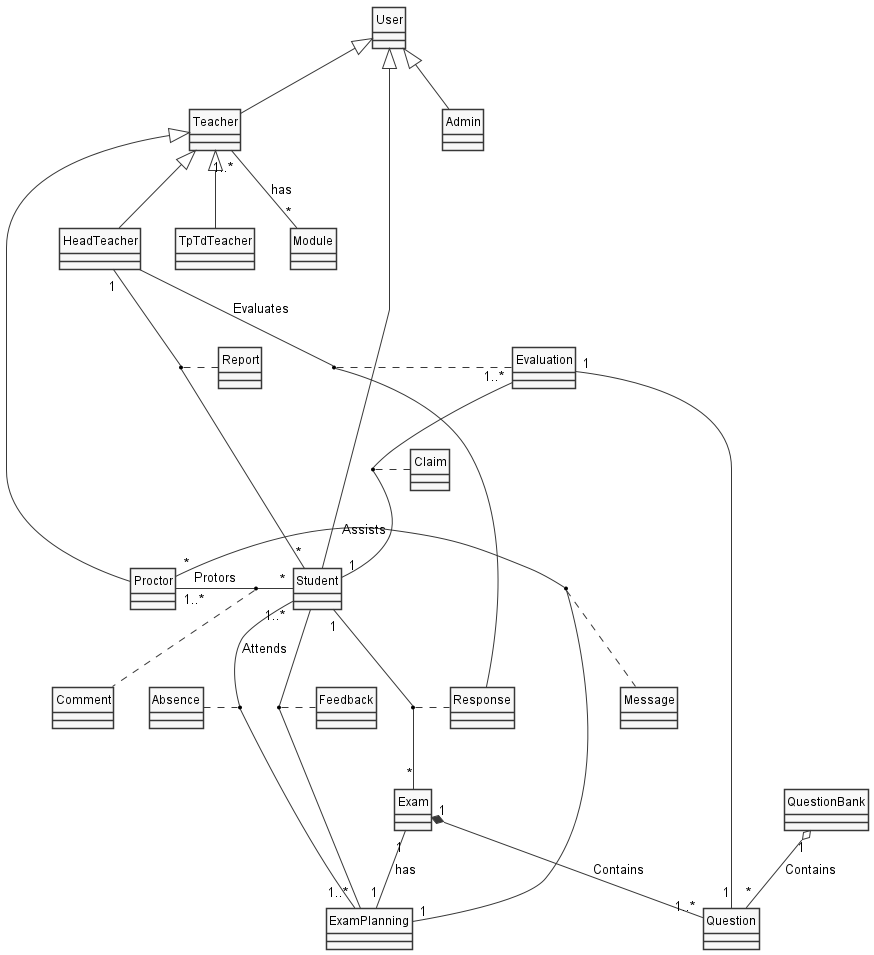
\includegraphics[width=\textwidth]{images/DCD}
        \caption{Domain class diagram}
    \end{figure}


    \begin{figure}
        \section{Conception class diagram}
        \raggedright Defines the conceptual classes with details, specifying the methods and the visibility of both fields and methods.
        \linebreak
        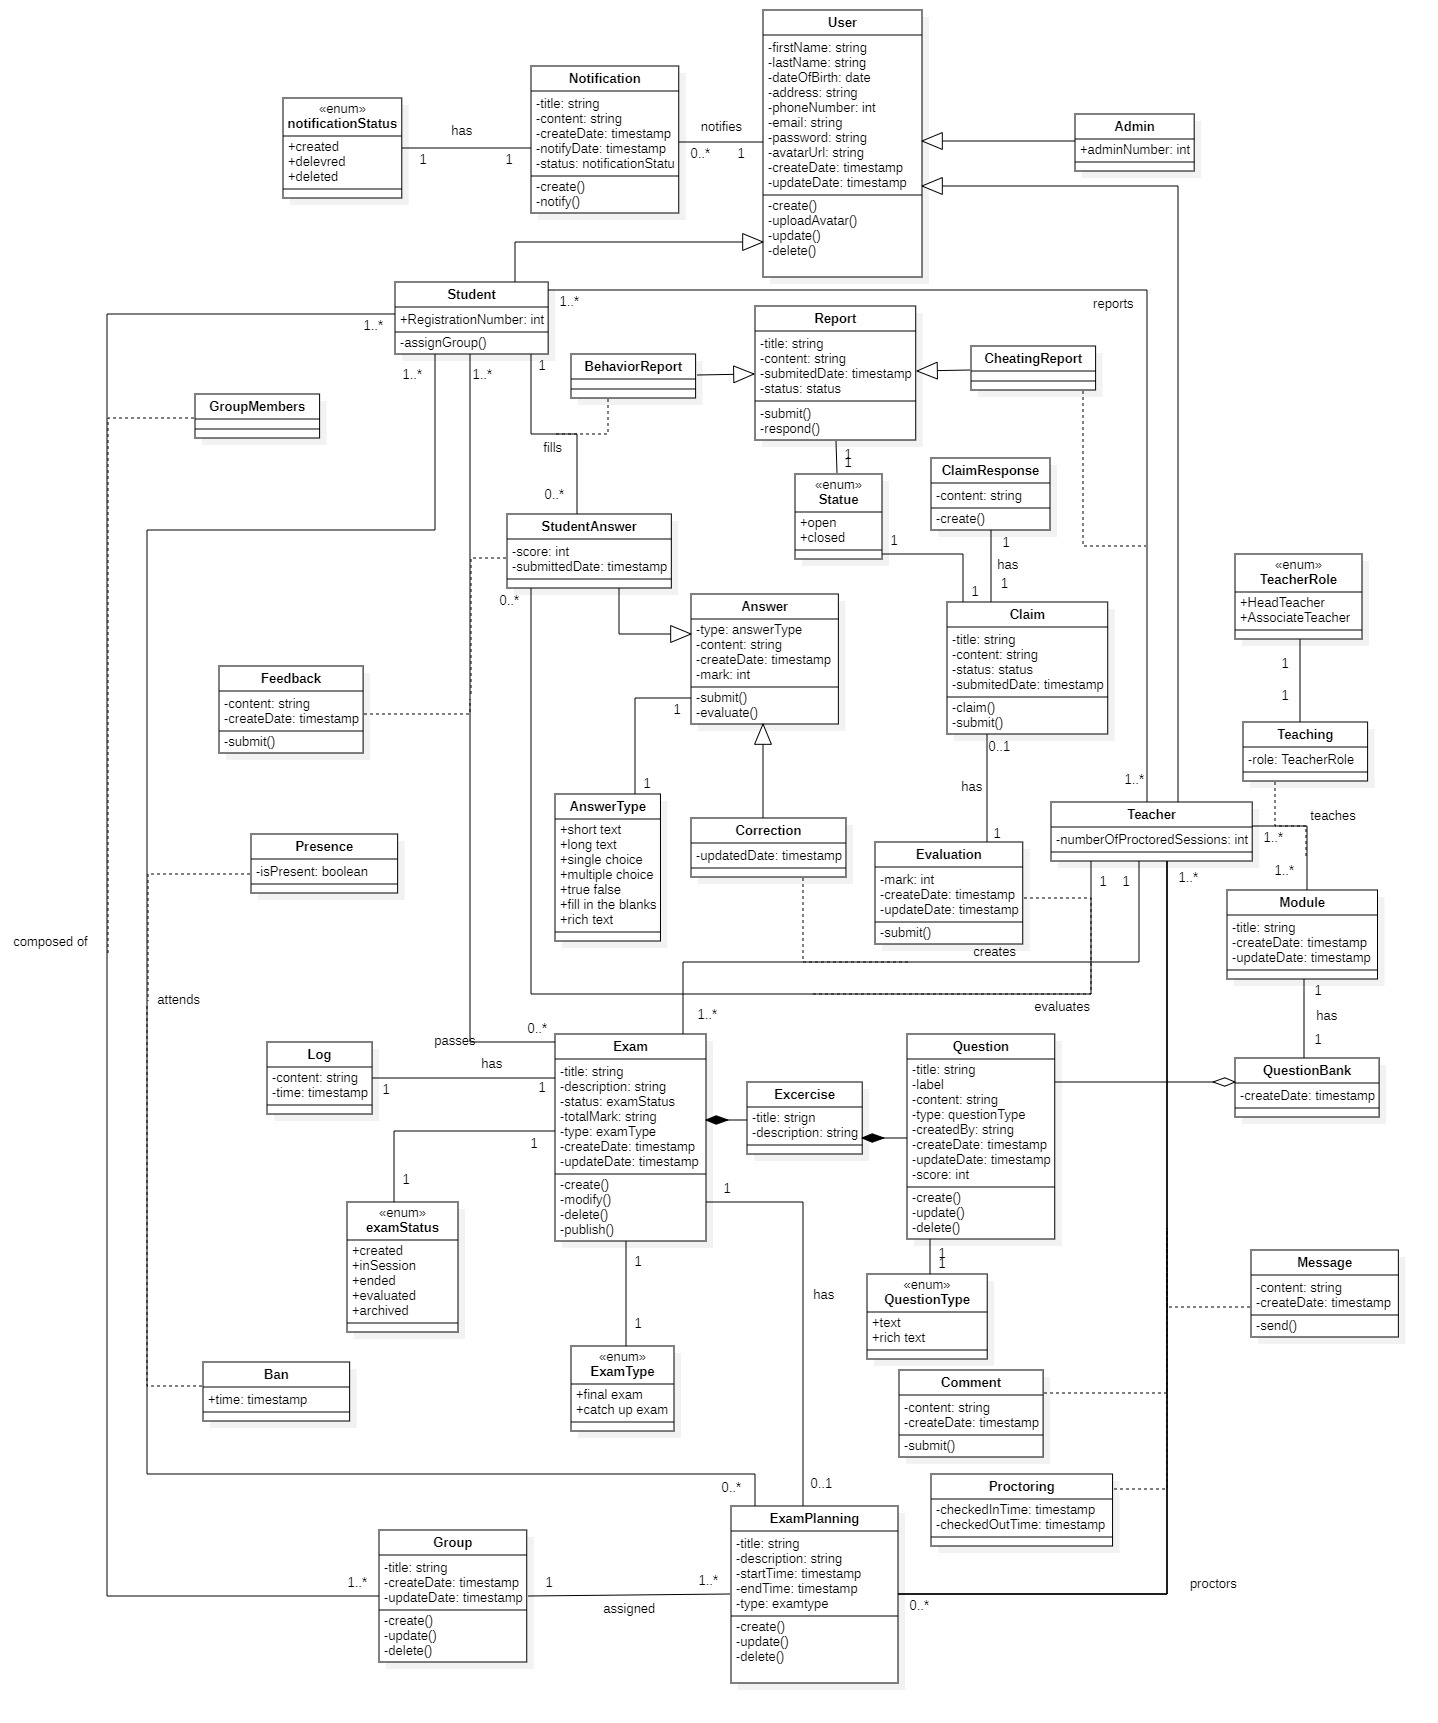
\includegraphics[width=\textwidth]{images/CCD}
        \caption{Conception class diagram}
    \end{figure}
    \clearpage


    \raggedright\section{Database}
    NoSQL, also referred to as “not only SQL”, “non-SQL”, is an approach to database design that enables the storage and querying of data outside the traditional structures found in relational databases.\linebreak
    \linebreak
    NoSQL databases invariably incorporate a flexible schema model and are designed to scale horizontally across many servers, which makes them appealing for large data volumes or application loads that exceed the capacity of a single server.
    The popularity of NoSQL has been driven by the following reasons:

    \begin{itemize}
        \item The pace of development with NoSQL databases can be much faster than with a SQL database.
        \item The structure of many different forms of data is more easily handled and evolved with a NoSQL database.
        \item The amount of data in many applications cannot be served affordably by a SQL database.
        \item The scale of traffic and need for zero downtime cannot be handled by SQL.
        \item New application paradigms can be more easily supported.
    \end{itemize}
    \linebreak
    Here are the four main types of NoSQL databases: \textbf{Key-Value Stores, Column-Oriented Databases, Graph Databases, Document Databases.}


    \subsubsection{MangoDB:}
    MongoDB is a document database. In our development for the OSES system, we had to choose a database that will be flexible for potential scalability. \linebreak
    The reason for that is because we want our system to be able to constantly change to serve the needs of our customers.

    So we used the nosql databases, which was designed for this purpose in the first place,
    And which stand for not only sql,
    \clearpage


    \subsection{Database schema:}
    \raggedright Shows the database tables and their relations and attributes.
    \begin{figure}[h]
        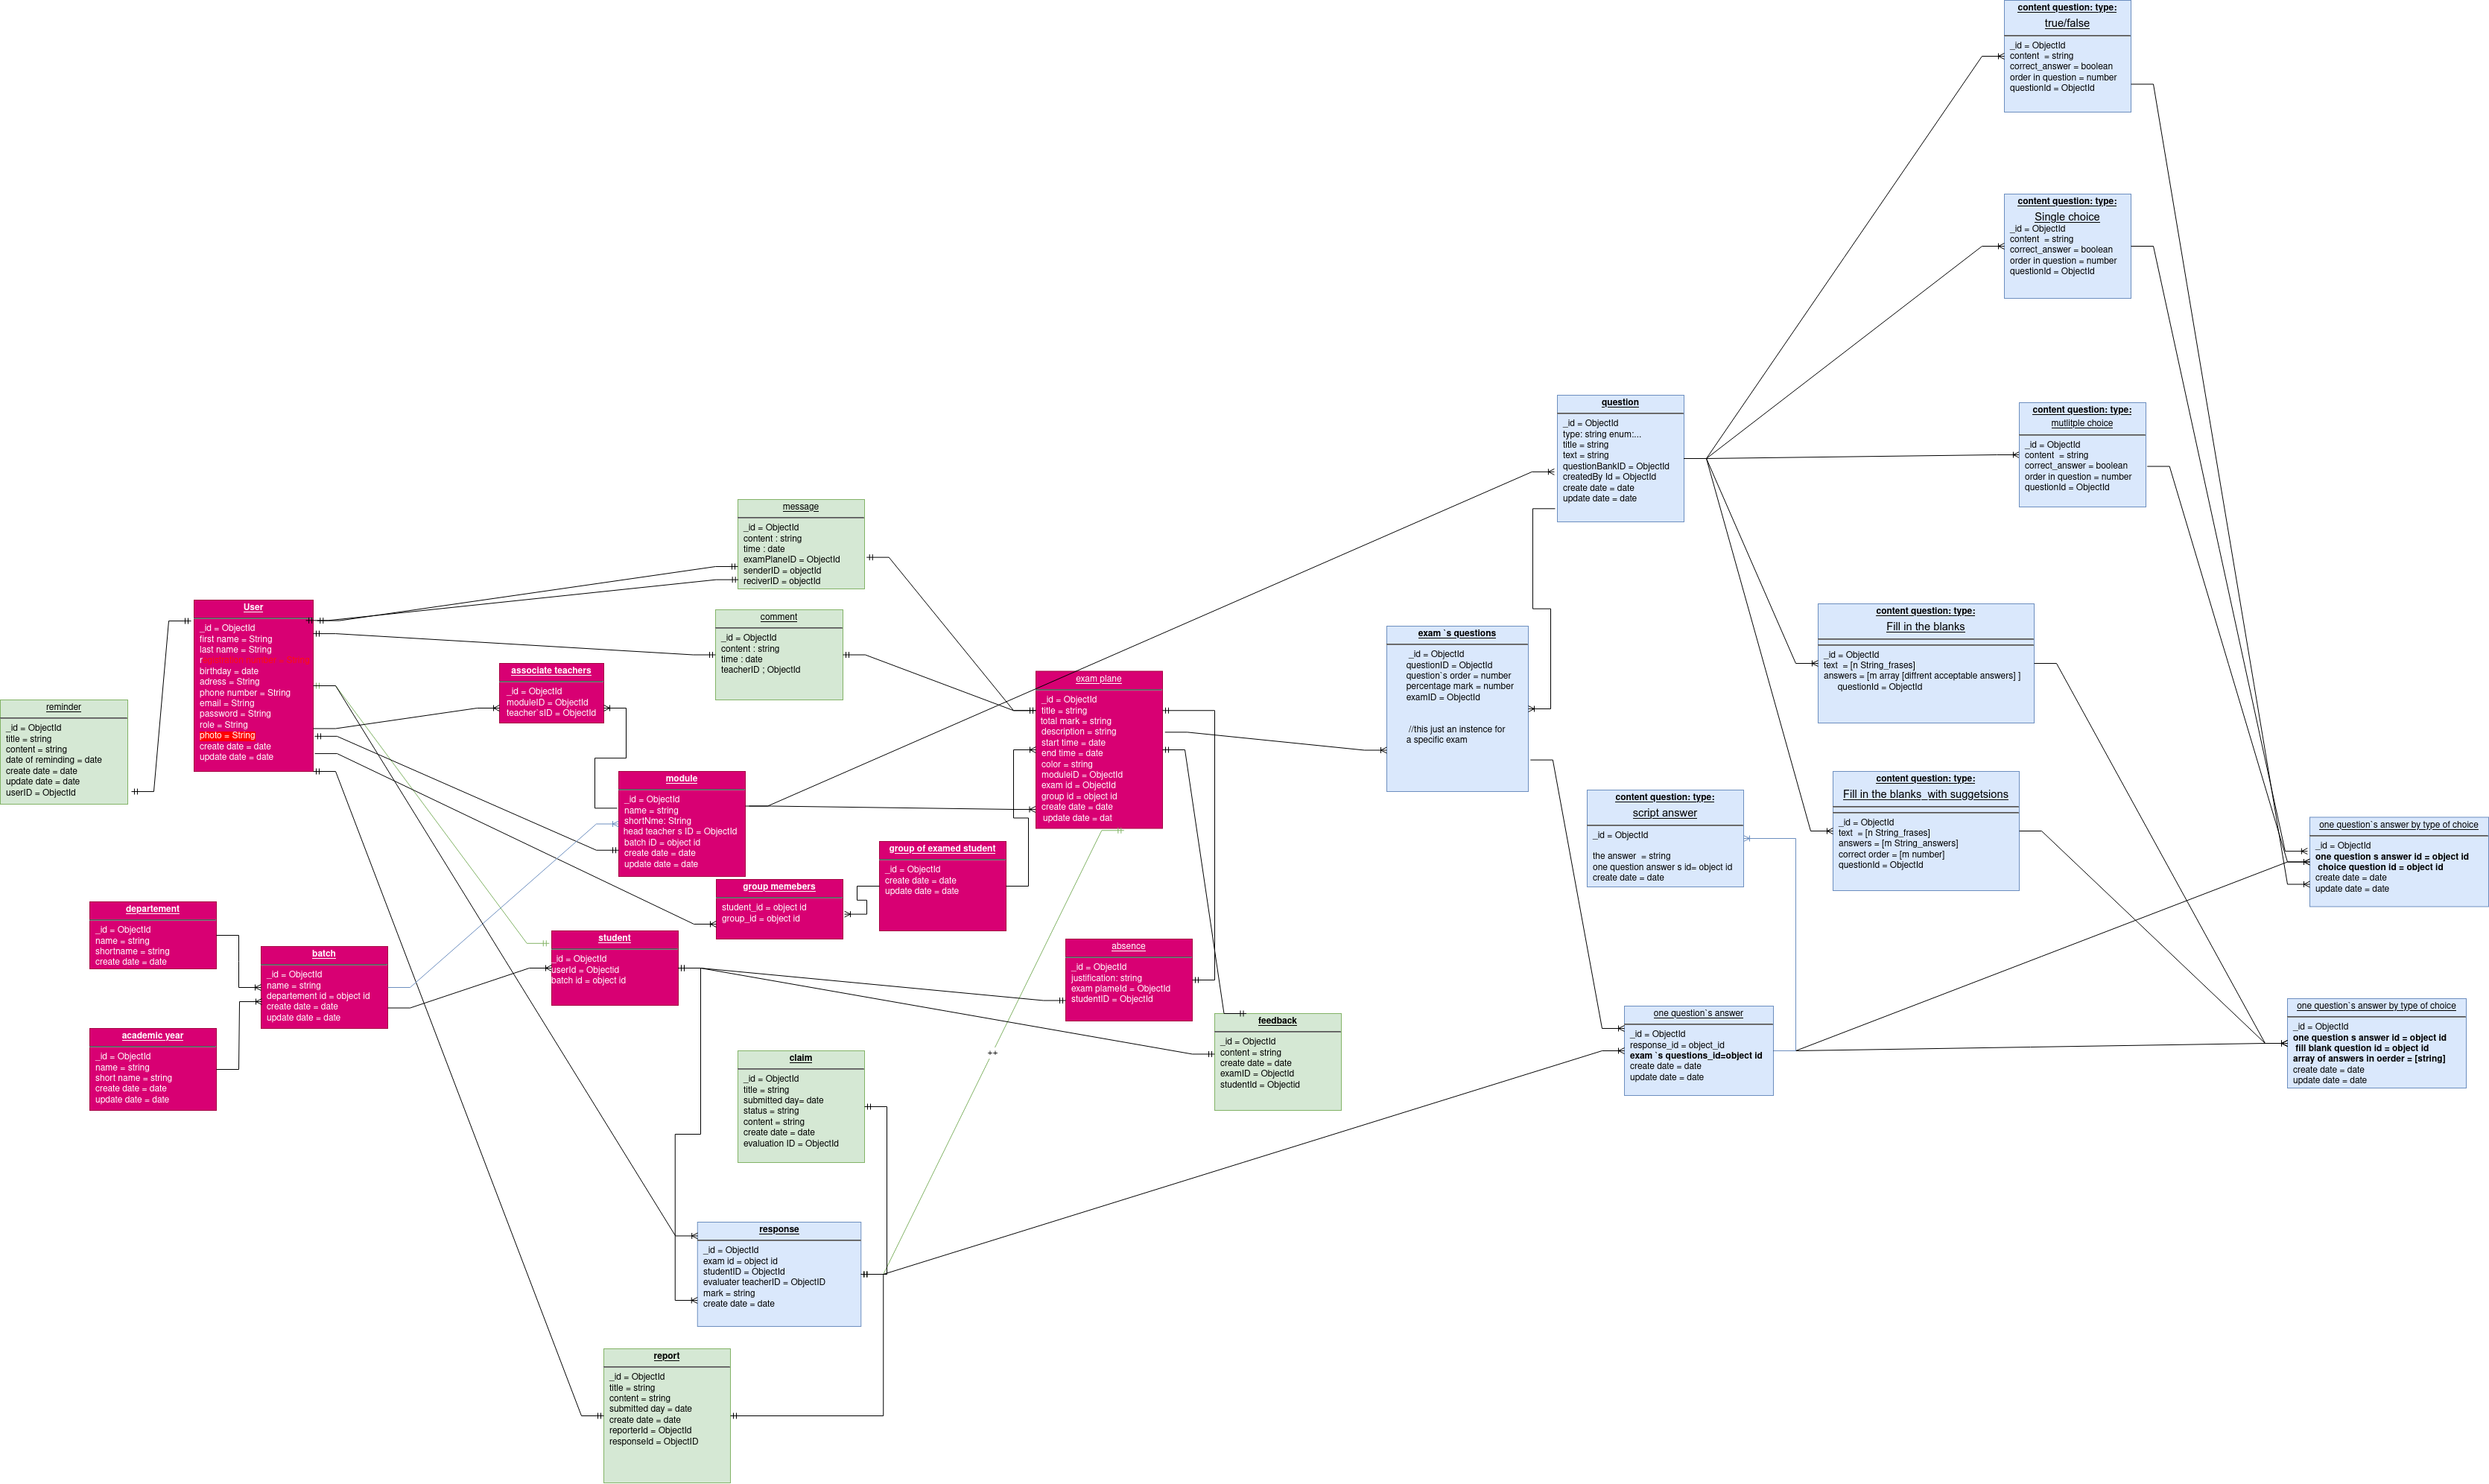
\includegraphics[width=\textwidth]{images/DbSchema}
        \caption{Database schema diagram}
    \end{figure}

    \raggedright\section{Conclusion}
    Throughout this chapter we walked through the conceptual aspects of our system, starting with the domain model in which entities are defined, followed by the domain class diagram; based on the domain class diagram we outlined what entities, attributes and methods make up our system.
    The first part of this chapter described how we envisioned our system and constructed its static aspect, but it was incomplete without speaking about how we implemented it to the physical level: the database, which is what the last part discusses, from transformation rules to the actual database diagram.
    In the next chapter and using the previous chapters as a foundation, we will cover the implementation part of our system, the technological choices, and the final results.


\end{document}